\documentclass{article}
\usepackage{tikz}

\begin{document}

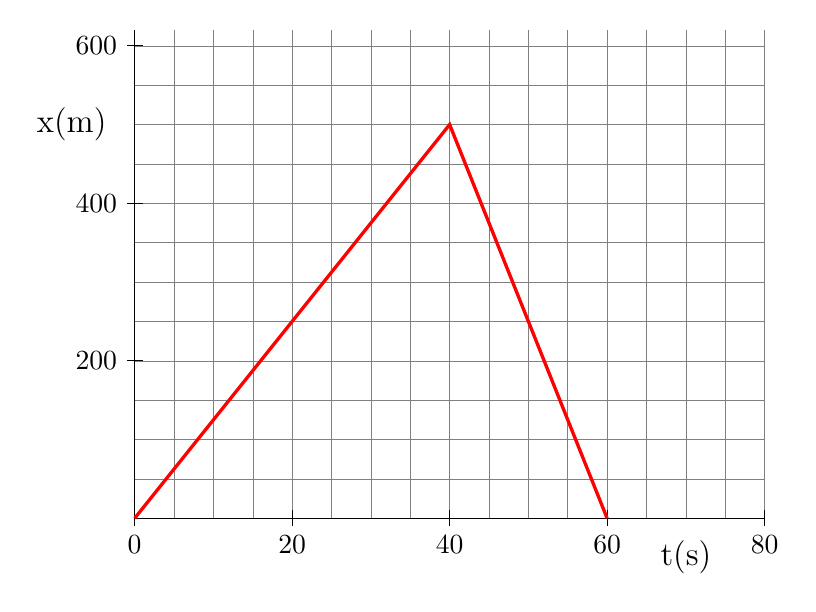
\begin{tikzpicture}[scale=0.1]
    \draw[step=5cm,gray,very thin] (0,0) grid (80,62);
    \draw (0,0) -- (80,0);
    \draw (0,0) -- (0,62);
    \foreach \x in {0,20,40,60,80}
    \draw (\x,1) -- (\x,-1) node[anchor=north] {\x};
    \node[font=\large] (X) at (70,-5) {t(s)};
    \foreach \y/\ytext in {20/200,40/400,60/600}
    \draw (1,\y) -- (-1,\y) node[anchor=east] {\ytext};
    \node[font=\large] (Y) at (-8,50) {x(m)};
    \draw[red,very thick] (0,0) -- (40,50) -- (60,0);
\end{tikzpicture}


\end{document}
